% Test Plan: Supporting Multi-homed DFS Servers (OSF-RFC 77.0)
% Copyright (C) 1996 Transarc Corporation - All rights reserved

\documentstyle[titlepage,psfig]{article}

\begin{document}

\title{Test Plan for OSF-RFC 77.0\\
Supporting Multi-homed DFS Servers}

\author{Transarc Corporation\\
\\
\copyright 1996 Transarc Corporation}
\date{May 1996}

\maketitle

%
% ------------------------------------------------------------------------
%

\section{INTRODUCTION}

This document describes a plan for testing the implementation
of OSF-RFC~77.0\footnote{S. Moyer. {\em Supporting Multi-Homed DFS Servers.}
OSF-RFC~77.0.  January 1996.}, DFS cache-manager (CM) support for
multi-homed servers.
The test suite presented is intended to supplement existing
cache-manager tests.  That is, it focuses only on testing the CM
code paths that implement multi-homed server support.

Section~\ref{sec:config} presents an overview of the DCE/DFS configuration
utilized by all tests in the suite.
Section~\ref{sec:suite} describes the test suite in detail.

It is assumed that the reader is familiar with the details of OSF-RFC~77.0.

%
% ------------------------------------------------------------------------
%

\section{TEST CONFIGURATION}
\label{sec:config}

All tests presume a DCE cell containing at least two DFS server
machines: $A$ and $B$.
Machine $A$ is a multi-homed host with (at least)
network-connections $A_{1}$ and $A_{2}$ that executes a file-server,
repserver and flserver; this flserver must be the only one in the cell.
Machine $B$ is a multi-homed host with (at least)
network-connections
$B_{1}$ and $B_{2}$ that executes a file-server and repserver.
Tests are executed on a client machine that is neither $A$ nor $B$.

Note that throughout this text, the names $A_{1}$, $A_{2}$, $B_{1}$
and $B_{2}$ refer to physical connections or connection-addresses as the
context dictates.

The DFS server machines $A$ and $B$ must be configured such that server
processes export bindings to CDS for only $A_{2}$ and $B_{2}$, respectively,
allowing other connections to be configured down as testing
requires.
Machine $A$'s FLDB and CDS (\mbox{\em.../self}) entries must
contain $A_{1}$ and $A_{2}$ only, while machine $B$'s FLDB entry
must contain $B_{1}$ only\footnote{Because servers on host $A$ are
configured to export $A_{2}$ only, $A_{1}$ will not automatically appear
in CDS; it must be put there manually.}.

For the machine executing the tests, CM server-preference ranks
must be set such that
$rank(A_{1}) < rank(B_{1}) < rank(A_{2})$.
Note that the rank of $B_{2}$ is irrelevant since $B_{2}$ does not
appear in the FLDB.

Finally, the file {\tt file.RW} must reside in a read-write fileset
located on $A$, and the file {\tt file.RO} must reside in a read-only
fileset with a replica located on $A$ and $B$ only.

Figure~\ref{fig:config} depicts the required configuration.
Note that $B_{2}$ does not appear since it is not used by the CM
to communicate with DFS servers on $B$.

\begin{figure}
\begin{center}
\leavevmode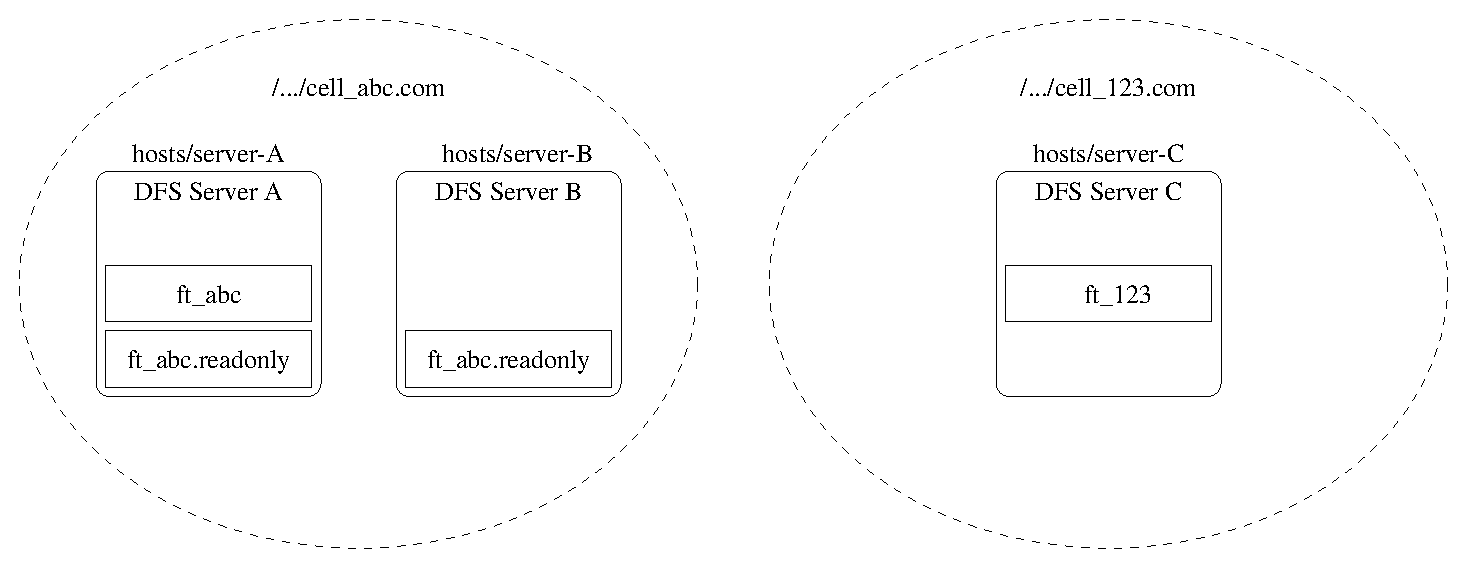
\psfig{file=config.ps,width=0.75\textwidth}
\caption{Multi-homed DFS Server Test Configuration}
\label{fig:config}
\end{center}
\end{figure}

This rather complex configuration is required so that the tests can
force failures to occur in a controlled fashion, thus generating predictable
results and allowing all code paths to be exercised.
Fortunately, the scripts which implement the tests described in
this document perform the required configuration.



%
% ------------------------------------------------------------------------
%

\section{TEST SUITE}
\label{sec:suite}

This section describes a collection of tests designed to exercise the
code paths that implement DFS cache-manager support for multi-homed servers.
All tests are presented in tabular form, with an action column and
one or more result columns.  Actions are performed from top to
bottom, with the action column representing a single iteration for
multi-phase tests (i.e.\ tests which iterate over the action column
multiple times).  Certain actions may only occur in certain phases; these
are labeled accordingly.  There is one result column for each iteration of
the action column.  Result columns represent correct results.

\subsection{Multi-server Binding}
\label{subsec:connbymhosts}

These tests exercise the CM function
{\tt cm\_ConnByMHosts() (cm\_Conn())}, the most commonly used of the
two server-binding functions.
{\tt cm\_ConnByMHosts()} attempts to get a binding for any one of
a set of servers, in accordance with the server-preference scheme;
i.e.\ addresses are tried for binding in rank order across the set of
all servers.

To exercise the complete range of multi-homed-server functionality,
both tests are designed to verify the correct behavior of
address fail-over, address revival and address acquisition.
In particular, address fail-over must occur in address-rank order,
address revival must be performed for servers marked as up or down,
and the address acquisition mechanisms must track changes in the
address sources (FLDB and CDS).  Note that these tests verify address
acquisition from the FLDB (file-servers/repservers) only, and
then not the extended address-acquisition mechanism.

Figure~\ref{fig:connbymhosts2} depicts a test which
accesses the file {\tt file.RO} from the replicated fileset.
This test exercises {\tt cm\_ConnByMHosts()} for two servers.

Figure~\ref{fig:connbymhosts1} depicts a test which
accesses the file {\tt file.RW} from the read-write fileset.
This test exercises {\tt cm\_ConnByMHosts()} for the case where only
a single server is specified.

It should be noted that multi-homed-server related activity other
than that listed in the test results may be observed.  This can
occur if various CM background threads execute during the course
of a test.

\begin{figure}
\begin{tabular}{|p{1.4in}|p{0.9in}|p{0.9in}|p{0.9in}|}
\hline
\multicolumn{4}{|c|}{Multi-server Binding --- Replicated Fileset Access} \\
\hline
\hline
 & \multicolumn{3}{c|}{Result} \\ \cline{2-4}
\multicolumn{1}{|c|}{Action} & \multicolumn{1}{c|}{Phase A} &
    \multicolumn{1}{c|}{Phase B} & \multicolumn{1}{c|}{Phase C} \\
%
\hline
{\raggedright cm~checkf} & & & \\
%
\hline
{\raggedright cat~file.RO;\\cm~flush~file.RO} &
{\raggedright access via $A_{1}$} &
{\raggedright access via $B_{1}$} &
{\raggedright access via $A_{1}$} \\
%
\hline
{\raggedright configure $A_{1}$ down} & & & \\
%
\hline
{\raggedright cat~file.RO;\\cm~flush~file.RO} &
{\raggedright $A_{1}$ fail-over;\\access via $B_{1}$} &
{\raggedright no fail-over;\\access via $B_{1}$} &
{\raggedright $A_{1}$ fail-over;\\access via $B_{1}$} \\
%
\hline
{\raggedright configure $B_{1}$ down} & & & \\
%
\hline
{\raggedright cat~file.RO;\\cm~flush~file.RO} &
{\raggedright FX $B$ down;\\access via $A_{2}$} &
{\raggedright FX $B$ down;\\access via $A_{2}$} &
{\raggedright FX $B$ down;\\access via $A_{2}$} \\
%
\hline
{\raggedright configure $B_{1}$ up} & & & \\
%
\hline
{\raggedright sleep dead-server poll time} &
{\raggedright FX $B$ back up} &
{\raggedright FX $B$ back up} &
{\raggedright FX $B$ back up} \\
%
\hline
{\raggedright cat~file.RO;\\cm~flush~file.RO} &
{\raggedright access via $B_{1}$} &
{\raggedright access via $B_{1}$} &
{\raggedright access via $B_{1}$} \\
%
\hline
{\raggedright configure $A_{1}$ up} & & & \\
%
\hline
{\raggedright {\bf A/C}: sleep live-server poll time} &
{\raggedright revival of $A_{1}$} &
 &
{\raggedright revival of $A_{1}$} \\
%
\hline
{\raggedright cat~file.RO;\\cm~flush~file.RO} &
{\raggedright access via $A_{1}$} &
{\raggedright access via $B_{1}$} &
{\raggedright access via $A_{1}$} \\
%
\hline
{\raggedright
  {\bf A}: fts~eds~$A_{1}$~-rm;\\
  {\bf B}: fts~eds~$A_{2}$~-add~$A_{1}$;\\cm~setpref~$A_{1}$} & & & \\
%
\hline
\end{tabular}
\caption{Two server test of cm\_ConnByMHosts() (cm\_Conn())}
\label{fig:connbymhosts2}
\end{figure}



\begin{figure}
\begin{tabular}{|p{1.4in}|p{0.9in}|p{0.9in}|p{0.9in}|}
\hline
\multicolumn{4}{|c|}{Multi-server Binding --- Read-Write Fileset Access} \\
\hline
\hline
 & \multicolumn{3}{c|}{Result} \\ \cline{2-4}
\multicolumn{1}{|c|}{Action} & \multicolumn{1}{c|}{Phase A} &
    \multicolumn{1}{c|}{Phase B} & \multicolumn{1}{c|}{Phase C} \\
%
\hline
{\raggedright cm~checkf} & & & \\
%
\hline
{\raggedright cat~file.RW;\\cm~flush~file.RW} &
{\raggedright access via $A_{1}$} &
{\raggedright access via $A_{1}$} &
{\raggedright access via $A_{1}$} \\
%
\hline
{\raggedright configure $A_{1}$ down} & & & \\
%
\hline
%{\raggedright
%  {\bf A/C}: cat~file.RW;\\cm~flush~file.RW \\
%  {\bf B}: cat~file.RW} &
{\raggedright cat~file.RW;\\cm~flush~file.RW} &
{\raggedright $A_{1}$ fail-over;\\access via $A_{2}$} &
{\raggedright FX $A$ down;\\not accessible} &
{\raggedright $A_{1}$ fail-over;\\access via $A_{2}$} \\
%
\hline
{\raggedright configure $A_{1}$ up} & & & \\
%
\hline
{\raggedright
  {\bf A/C}: sleep live-server poll time\\
  {\bf B}: sleep dead-server poll time} &
{\raggedright revival of $A_{1}$} &
{\raggedright FX $A$ back up} &
{\raggedright revival of $A_{1}$} \\
%
\hline
{\raggedright cat~file.RW;\\cm~flush~file.RW} &
{\raggedright access via $A_{1}$} &
{\raggedright access via $A_{1}$} &
{\raggedright access via $A_{1}$} \\
%
\hline
{\raggedright
  {\bf A}: fts~eds~$A_{2}$~-rm\\
  {\bf B}: fts~eds~$A_{1}$~-add~$A_{2}$;\\cm~setpref~$A_{2}$} & & & \\
%
\hline
\end{tabular}
\caption{Single server test of cm\_ConnByMHosts() (cm\_Conn())}
\label{fig:connbymhosts1}
\end{figure}



\subsection{Single-server Binding}
\label{subsec:connbyhost}

This test exercises the CM function
{\tt cm\_ConnByHost()}, which attempts to get a binding for a particular
server in accordance with the server-preference scheme;
i.e.\ addresses are tried for binding in rank order.

Once again, to exercise the complete range of multi-homed-server
functionality,
the test is designed to verify the correct behavior of
address fail-over, address revival and address acquisition.
As with the previous tests, this test verifies address
acquisition from the FLDB (file-servers/repservers) only, and
then not the extended address-acquisition mechanism.

Figure~\ref{fig:connbyhost} depicts the test, which performs
server status checks in order to generate server pings.
Pinging a server, via an {\tt AFS\_GetTime()} RPC, is one of the
few CM functions which employs {\tt cm\_ConnByHost()}.  Note
that the test maintains an open token for the
file {\tt file.RW} located on the
server being pinged; this is necessary in order for the CM
to consider the server ``interesting enough'' to ping.

Again it should be noted that multi-homed-server related activity other
than that listed in the test results may be observed if
various CM background threads execute during the course
of the test.


\begin{figure}
\begin{tabular}{|p{1.4in}|p{0.9in}|p{0.9in}|p{0.9in}|}
\hline
\multicolumn{4}{|c|}{Single-server Binding --- Server Status Check} \\
\hline
\hline
 & \multicolumn{3}{c|}{Result} \\ \cline{2-4}
\multicolumn{1}{|c|}{Action} & \multicolumn{1}{c|}{Phase A} &
    \multicolumn{1}{c|}{Phase B} & \multicolumn{1}{c|}{Phase C} \\
%
\hline
{\raggedright cm~checkf} & & & \\
%
\hline
{\raggedright open~file.RW} & & & \\
%
\hline
{\raggedright cm~statservers} &
{\raggedright ping via $A_{1}$} &
{\raggedright ping via $A_{1}$} &
{\raggedright ping via $A_{1}$} \\
%
\hline
{\raggedright configure $A_{1}$ down} & & & \\
%
\hline
{\raggedright cm~statservers} &
{\raggedright $A_{1}$ fail-over;\\ping via $A_{2}$} &
{\raggedright FX $A$ down} &
{\raggedright $A_{1}$ fail-over;\\ping via $A_{2}$} \\
%
\hline
{\raggedright configure $A_{1}$ up} & & & \\
%
\hline
{\raggedright
  {\bf A/C}: sleep live-server poll time\\
  {\bf B}: sleep dead-server poll time;\\close~file.RW;\\open~file.RW} &
{\raggedright revival of $A_{1}$} &
{\raggedright FX $A$ back up} &
{\raggedright revival of $A_{1}$} \\
%
\hline
{\raggedright cm~statservers} &
{\raggedright ping via $A_{1}$} &
{\raggedright ping via $A_{1}$} &
{\raggedright ping via $A_{1}$} \\
%
\hline
{\raggedright close~file.RW} & & & \\
%
\hline
{\raggedright
  {\bf A}: fts~eds~$A_{2}$~-rm;\\
  {\bf B}: fts~eds~$A_{1}$~-add~$A_{2}$;\\cm~setpref~$A_{2}$} & & & \\
%
\hline
\end{tabular}
\caption{Test of cm\_ConnByHost()}
\label{fig:connbyhost}
\end{figure}



\subsection{CDS Address Acquisition}
\label{subsec:flserver-addr}

This test exercises the flserver address-acquisition mechanism, which
is not exercised by the binding-function tests.  Essentially, it
verifies that the CM tracks flserver address changes in the CDS.

Figure~\ref{fig:floc} depicts the test, which performs fileset
location checks in order to generate flserver RPCs.  Note
that the ``cm~checkfilesets'' command issued prior to each ``cm~whereis''
command forces the CM both to update flserver addresses from
the CDS, and to go to the flserver for current information.


\begin{figure}
\begin{tabular}{|p{1.4in}|p{0.9in}|p{0.9in}|p{0.9in}|}
\hline
\multicolumn{4}{|c|}{CDS Address Acquisition --- Fileset Location Check} \\
\hline
\hline
 & \multicolumn{3}{c|}{Result} \\ \cline{2-4}
\multicolumn{1}{|c|}{Action} & \multicolumn{1}{c|}{Phase A} &
    \multicolumn{1}{c|}{Phase B} & \multicolumn{1}{c|}{Phase C} \\
%
\hline
{\raggedright cm~checkf;\\cm~whereis~/:/} &
{\raggedright lookup via $A_{1}$} &
{\raggedright lookup via $A_{1}$} &
{\raggedright lookup via $A_{1}$} \\
%
\hline
{\raggedright configure $A_{1}$ down} & & & \\
%
\hline
{\raggedright cm~checkf;\\cm~whereis~/:/} &
{\raggedright $A_{1}$ fail-over;\\lookup via $A_{2}$} &
{\raggedright FL $A$ down;\\lookup fails} &
{\raggedright $A_{1}$ fail-over;\\lookup via $A_{2}$} \\
%
\hline
{\raggedright configure $A_{1}$ up} & & & \\
%
\hline
{\raggedright
  {\bf A/C}: sleep live-server poll time\\
  {\bf B}: sleep dead-server poll time} &
{\raggedright revival of $A_{1}$} &
{\raggedright FL $A$ back up} &
{\raggedright revival of $A_{1}$} \\
%
\hline
{\raggedright cm~checkf;\\cm~whereis~/:/} &
{\raggedright lookup via $A_{1}$} &
{\raggedright lookup via $A_{1}$} &
{\raggedright lookup via $A_{1}$} \\
%
\hline
{\raggedright
  {\bf A}: rm $A_{2}$ from CDS\\
  {\bf B}: add $A_{2}$ to CDS;\\cm~setpref~$A_{2}$} & & & \\
%
\hline
\end{tabular}
\caption{Test of flserver address-acquisition from CDS}
\label{fig:floc}
\end{figure}




%
% ------------------------------------------------------------------------
%

\section{FUTURE TESTS}

The current tests in the suite exercise the vast majority of the code
paths that implement multi-homed server support.
However, a few additional tests may be added in the future to complete
coverage.

\subsection{Extended FLDB Address Acquisition}
\label{subsec:fldbxtra-addr}

As discussed in OSF-RFC~77.0, an extended file-server/repserver
address-acquisition mechanism is required to handle the case where
the address list provided in
{\tt cm\_InstallVolumeEntry()} (obtained via
{\tt VL\_GetEntryBy*()}) does not contain all
file-server/repserver addresses listed in the FLDB.

A test is required to exercise this mechanism, which is not exercised
by the binding-function tests.


\subsection{Fail-over Count Adherence}

The cache-manager maintains a per-server fail-over count indicating the
number of consecutive failed RPCs to each server.
When a server's fail-over count reaches a predefined upper-bound, the
server is declared down.

A test is required which varies the maximum fail-over count in
order to exercise this logic.


\subsection{Address Override}

The DCE RPC may change a binding's address to comply with that used by
the underlying transport layer.
The cache-manager reacts to such changes by overriding the preferred
server address (lowest rank) in favor of that in the binding.

A test is required which exercises this override path.

%
% ------------------------------------------------------------------------
%

\end{document}
